
%% bare_conf.tex
%% V1.4b
%% 2015/08/26
%% by Michael Shell
%% See:
%% http://www.michaelshell.org/
%% for current contact information.
%%
%% This is a skeleton file demonstrating the use of IEEEtran.cls
%% (requires IEEEtran.cls version 1.8b or later) with an IEEE
%% conference paper.
%%
%% Support sites:
%% http://www.michaelshell.org/tex/ieeetran/
%% http://www.ctan.org/pkg/ieeetran
%% and
%% http://www.ieee.org/

%%*************************************************************************
%% Legal Notice:
%% This code is offered as-is without any warranty either expressed or
%% implied; without even the implied warranty of MERCHANTABILITY or
%% FITNESS FOR A PARTICULAR PURPOSE! 
%% User assumes all risk.
%% In no event shall the IEEE or any contributor to this code be liable for
%% any damages or losses, including, but not limited to, incidental,
%% consequential, or any other damages, resulting from the use or misuse
%% of any information contained here.
%%
%% All comments are the opinions of their respective authors and are not
%% necessarily endorsed by the IEEE.
%%
%% This work is distributed under the LaTeX Project Public License (LPPL)
%% ( http://www.latex-project.org/ ) version 1.3, and may be freely used,
%% distributed and modified. A copy of the LPPL, version 1.3, is included
%% in the base LaTeX documentation of all distributions of LaTeX released
%% 2003/12/01 or later.
%% Retain all contribution notices and credits.
%% ** Modified files should be clearly indicated as such, including  **
%% ** renaming them and changing author support contact information. **
%%*************************************************************************


% *** Authors should verify (and, if needed, correct) their LaTeX system  ***
% *** with the testflow diagnostic prior to trusting their LaTeX platform ***
% *** with production work. The IEEE's font choices and paper sizes can   ***
% *** trigger bugs that do not appear when using other class files.       ***                          ***
% The testflow support page is at:
% http://www.michaelshell.org/tex/testflow/



\documentclass[conference]{IEEEtran}
% Some Computer Society conferences also require the compsoc mode option,
% but others use the standard conference format.
%
% If IEEEtran.cls has not been installed into the LaTeX system files,
% manually specify the path to it like:
% \documentclass[conference]{../sty/IEEEtran}





% Some very useful LaTeX packages include:
% (uncomment the ones you want to load)


% *** MISC UTILITY PACKAGES ***
%
%\usepackage{ifpdf}
% Heiko Oberdiek's ifpdf.sty is very useful if you need conditional
% compilation based on whether the output is pdf or dvi.
% usage:
% \ifpdf
%   % pdf code
% \else
%   % dvi code
% \fi
% The latest version of ifpdf.sty can be obtained from:
% http://www.ctan.org/pkg/ifpdf
% Also, note that IEEEtran.cls V1.7 and later provides a builtin
% \ifCLASSINFOpdf conditional that works the same way.
% When switching from latex to pdflatex and vice-versa, the compiler may
% have to be run twice to clear warning/error messages.






% *** CITATION PACKAGES ***
%
%\usepackage{cite}
% cite.sty was written by Donald Arseneau
% V1.6 and later of IEEEtran pre-defines the format of the cite.sty package
% \cite{} output to follow that of the IEEE. Loading the cite package will
% result in citation numbers being automatically sorted and properly
% "compressed/ranged". e.g., [1], [9], [2], [7], [5], [6] without using
% cite.sty will become [1], [2], [5]--[7], [9] using cite.sty. cite.sty's
% \cite will automatically add leading space, if needed. Use cite.sty's
% noadjust option (cite.sty V3.8 and later) if you want to turn this off
% such as if a citation ever needs to be enclosed in parenthesis.
% cite.sty is already installed on most LaTeX systems. Be sure and use
% version 5.0 (2009-03-20) and later if using hyperref.sty.
% The latest version can be obtained at:
% http://www.ctan.org/pkg/cite
% The documentation is contained in the cite.sty file itself.






% *** GRAPHICS RELATED PACKAGES ***
%
\ifCLASSINFOpdf
  \usepackage[pdftex]{graphicx}
  % declare the path(s) where your graphic files are
  % \graphicspath{{../pdf/}{../jpeg/}}
  \graphicspath{{images/}}
  % and their extensions so you won't have to specify these with
  % every instance of \includegraphics
  % \DeclareGraphicsExtensions{.pdf,.jpeg,.png}
\else
  % or other class option (dvipsone, dvipdf, if not using dvips). graphicx
  % will default to the driver specified in the system graphics.cfg if no
  % driver is specified.
  \usepackage[dvips]{graphicx}
  % declare the path(s) where your graphic files are
  % \graphicspath{{../eps/}}
  \graphicspath{{images/}}
  % and their extensions so you won't have to specify these with
  % every instance of \includegraphics
  % \DeclareGraphicsExtensions{.eps}
\fi
% graphicx was written by David Carlisle and Sebastian Rahtz. It is
% required if you want graphics, photos, etc. graphicx.sty is already
% installed on most LaTeX systems. The latest version and documentation
% can be obtained at: 
% http://www.ctan.org/pkg/graphicx
% Another good source of documentation is "Using Imported Graphics in
% LaTeX2e" by Keith Reckdahl which can be found at:
% http://www.ctan.org/pkg/epslatex
%
% latex, and pdflatex in dvi mode, support graphics in encapsulated
% postscript (.eps) format. pdflatex in pdf mode supports graphics
% in .pdf, .jpeg, .png and .mps (metapost) formats. Users should ensure
% that all non-photo figures use a vector format (.eps, .pdf, .mps) and
% not a bitmapped formats (.jpeg, .png). The IEEE frowns on bitmapped formats
% which can result in "jaggedy"/blurry rendering of lines and letters as
% well as large increases in file sizes.
%
% You can find documentation about the pdfTeX application at:
% http://www.tug.org/applications/pdftex





% *** MATH PACKAGES ***
%
\usepackage{amsmath}
% A popular package from the American Mathematical Society that provides
% many useful and powerful commands for dealing with mathematics.
%
% Note that the amsmath package sets \interdisplaylinepenalty to 10000
% thus preventing page breaks from occurring within multiline equations. Use:
\interdisplaylinepenalty=2500
% after loading amsmath to restore such page breaks as IEEEtran.cls normally
% does. amsmath.sty is already installed on most LaTeX systems. The latest
% version and documentation can be obtained at:
% http://www.ctan.org/pkg/amsmath





% *** SPECIALIZED LIST PACKAGES ***
%
%\usepackage{algorithmic}
% algorithmic.sty was written by Peter Williams and Rogerio Brito.
% This package provides an algorithmic environment fo describing algorithms.
% You can use the algorithmic environment in-text or within a figure
% environment to provide for a floating algorithm. Do NOT use the algorithm
% floating environment provided by algorithm.sty (by the same authors) or
% algorithm2e.sty (by Christophe Fiorio) as the IEEE does not use dedicated
% algorithm float types and packages that provide these will not provide
% correct IEEE style captions. The latest version and documentation of
% algorithmic.sty can be obtained at:
% http://www.ctan.org/pkg/algorithms
% Also of interest may be the (relatively newer and more customizable)
% algorithmicx.sty package by Szasz Janos:
% http://www.ctan.org/pkg/algorithmicx




% *** ALIGNMENT PACKAGES ***
%
%\usepackage{array}
% Frank Mittelbach's and David Carlisle's array.sty patches and improves
% the standard LaTeX2e array and tabular environments to provide better
% appearance and additional user controls. As the default LaTeX2e table
% generation code is lacking to the point of almost being broken with
% respect to the quality of the end results, all users are strongly
% advised to use an enhanced (at the very least that provided by array.sty)
% set of table tools. array.sty is already installed on most systems. The
% latest version and documentation can be obtained at:
% http://www.ctan.org/pkg/array


% IEEEtran contains the IEEEeqnarray family of commands that can be used to
% generate multiline equations as well as matrices, tables, etc., of high
% quality.




% *** SUBFIGURE PACKAGES ***
\ifCLASSOPTIONcompsoc
  \usepackage[caption=false,font=normalsize,labelfont=sf,textfont=sf]{subfig}
\else
  \usepackage[caption=false,font=footnotesize]{subfig}
\fi
% subfig.sty, written by Steven Douglas Cochran, is the modern replacement
% for subfigure.sty, the latter of which is no longer maintained and is
% incompatible with some LaTeX packages including fixltx2e. However,
% subfig.sty requires and automatically loads Axel Sommerfeldt's caption.sty
% which will override IEEEtran.cls' handling of captions and this will result
% in non-IEEE style figure/table captions. To prevent this problem, be sure
% and invoke subfig.sty's "caption=false" package option (available since
% subfig.sty version 1.3, 2005/06/28) as this is will preserve IEEEtran.cls
% handling of captions.
% Note that the Computer Society format requires a larger sans serif font
% than the serif footnote size font used in traditional IEEE formatting
% and thus the need to invoke different subfig.sty package options depending
% on whether compsoc mode has been enabled.
%
% The latest version and documentation of subfig.sty can be obtained at:
% http://www.ctan.org/pkg/subfig




% *** FLOAT PACKAGES ***
%
%\usepackage{fixltx2e}
% fixltx2e, the successor to the earlier fix2col.sty, was written by
% Frank Mittelbach and David Carlisle. This package corrects a few problems
% in the LaTeX2e kernel, the most notable of which is that in current
% LaTeX2e releases, the ordering of single and double column floats is not
% guaranteed to be preserved. Thus, an unpatched LaTeX2e can allow a
% single column figure to be placed prior to an earlier double column
% figure.
% Be aware that LaTeX2e kernels dated 2015 and later have fixltx2e.sty's
% corrections already built into the system in which case a warning will
% be issued if an attempt is made to load fixltx2e.sty as it is no longer
% needed.
% The latest version and documentation can be found at:
% http://www.ctan.org/pkg/fixltx2e


%\usepackage{stfloats}
% stfloats.sty was written by Sigitas Tolusis. This package gives LaTeX2e
% the ability to do double column floats at the bottom of the page as well
% as the top. (e.g., "\begin{figure*}[!b]" is not normally possible in
% LaTeX2e). It also provides a command:
%\fnbelowfloat
% to enable the placement of footnotes below bottom floats (the standard
% LaTeX2e kernel puts them above bottom floats). This is an invasive package
% which rewrites many portions of the LaTeX2e float routines. It may not work
% with other packages that modify the LaTeX2e float routines. The latest
% version and documentation can be obtained at:
% http://www.ctan.org/pkg/stfloats
% Do not use the stfloats baselinefloat ability as the IEEE does not allow
% \baselineskip to stretch. Authors submitting work to the IEEE should note
% that the IEEE rarely uses double column equations and that authors should try
% to avoid such use. Do not be tempted to use the cuted.sty or midfloat.sty
% packages (also by Sigitas Tolusis) as the IEEE does not format its papers in
% such ways.
% Do not attempt to use stfloats with fixltx2e as they are incompatible.
% Instead, use Morten Hogholm'a dblfloatfix which combines the features
% of both fixltx2e and stfloats:
%
% \usepackage{dblfloatfix}
% The latest version can be found at:
% http://www.ctan.org/pkg/dblfloatfix




% *** PDF, URL AND HYPERLINK PACKAGES ***
%
%\usepackage{url}
% url.sty was written by Donald Arseneau. It provides better support for
% handling and breaking URLs. url.sty is already installed on most LaTeX
% systems. The latest version and documentation can be obtained at:
% http://www.ctan.org/pkg/url
% Basically, \url{my_url_here}.




% hyperref
%
\usepackage[pdfpagemode={UseOutlines},bookmarks=true,bookmarksopen=true,
   bookmarksopenlevel=0,bookmarksnumbered=true,hypertexnames=false,
   colorlinks,linkcolor={blue},citecolor={blue},urlcolor={blue},
   pdfstartview={FitV},unicode,breaklinks=true]{hyperref}

% listing
%
\usepackage{listings,color}

\definecolor{dkgreen}{rgb}{0,0.6,0}
\definecolor{gray}{rgb}{0.5,0.5,0.5}
\definecolor{mauve}{rgb}{0.58,0,0.82}
\newcommand{\fsize}{\small}
%\newcommand{\fsize}{\tiny}
\newcommand{\tabsize}{4}

\lstset{frame=tb,
  language=C++,
%  aboveskip=0mm,
  belowskip=0mm,
  showstringspaces=false,
  columns=flexible,
  basicstyle={\fsize\ttfamily},
  numberstyle=\fsize\color{gray},
%  numbers=left,
  keywordstyle=\color{blue},
  commentstyle=\color{dkgreen},
  stringstyle=\color{mauve},
  breaklines=true,
  breakatwhitespace=true,
  tabsize=\tabsize
}

% *** Do not adjust lengths that control margins, column widths, etc. ***
% *** Do not use packages that alter fonts (such as pslatex).         ***
% There should be no need to do such things with IEEEtran.cls V1.6 and later.
% (Unless specifically asked to do so by the journal or conference you plan
% to submit to, of course. )


% correct bad hyphenation here
\hyphenation{op-tical net-works semi-conduc-tor}

\newcommand{\fref}[1]{\figurename~\ref{#1}}
\newcommand{\eref}[1]{(\ref{#1})}
\newcommand{\tref}[1]{\tablename~\ref{#1}}
\newcommand{\lref}[1]{LISTING~\ref{#1}}


\begin{document}
%
% paper title
% Titles are generally capitalized except for words such as a, an, and, as,
% at, but, by, for, in, nor, of, on, or, the, to and up, which are usually
% not capitalized unless they are the first or last word of the title.
% Linebreaks \\ can be used within to get better formatting as desired.
% Do not put math or special symbols in the title.
\title{Contour Trees Challenge Exercise Report}


% author names and affiliations
% use a multiple column layout for up to three different
% affiliations
\author{\IEEEauthorblockN{Yubo Zhi}
\IEEEauthorblockA{Imperial College London\\
MSc Analogue and Digital\\Integrated Circuit Design\\
Email: yz4116@ic.ac.uk}
\and
\IEEEauthorblockN{Jiayang Sun}
\IEEEauthorblockA{Imperial College London\\
MSc Analogue and Digital\\Integrated Circuit Design\\
Email: js11815@ic.ac.uk}
\and
\IEEEauthorblockN{Jiuxi Meng}
\IEEEauthorblockA{Imperial College London\\
MSc Analogue and Digital\\Integrated Circuit Design\\
Email: jm8415@ic.ac.uk}}

% conference papers do not typically use \thanks and this command
% is locked out in conference mode. If really needed, such as for
% the acknowledgment of grants, issue a \IEEEoverridecommandlockouts
% after \documentclass

% for over three affiliations, or if they all won't fit within the width
% of the page, use this alternative format:
% 
%\author{\IEEEauthorblockN{Michael Shell\IEEEauthorrefmark{1},
%Homer Simpson\IEEEauthorrefmark{2},
%James Kirk\IEEEauthorrefmark{3}, 
%Montgomery Scott\IEEEauthorrefmark{3} and
%Eldon Tyrell\IEEEauthorrefmark{4}}
%\IEEEauthorblockA{\IEEEauthorrefmark{1}School of Electrical and Computer Engineering\\
%Georgia Institute of Technology,
%Atlanta, Georgia 30332--0250\\ Email: see http://www.michaelshell.org/contact.html}
%\IEEEauthorblockA{\IEEEauthorrefmark{2}Twentieth Century Fox, Springfield, USA\\
%Email: homer@thesimpsons.com}
%\IEEEauthorblockA{\IEEEauthorrefmark{3}Starfleet Academy, San Francisco, California 96678-2391\\
%Telephone: (800) 555--1212, Fax: (888) 555--1212}
%\IEEEauthorblockA{\IEEEauthorrefmark{4}Tyrell Inc., 123 Replicant Street, Los Angeles, California 90210--4321}}




% use for special paper notices
%\IEEEspecialpapernotice{(Invited Paper)}




% make the title area
\maketitle

% As a general rule, do not put math, special symbols or citations
% in the abstract
\begin{abstract}
The course work is based on a contour tree library called "tourtre",
and a sample application named "simple". The aim of the exercise is to speed up the program and evaluate the performance of it. This short report will represent the result and have a small discussion and explanation. 
\end{abstract}

% no keywords




% For peer review papers, you can put extra information on the cover
% page as needed:
% \ifCLASSOPTIONpeerreview
% \begin{center} \bfseries EDICS Category: 3-BBND \end{center}
% \fi
%
% For peerreview papers, this IEEEtran command inserts a page break and
% creates the second title. It will be ignored for other modes.
\IEEEpeerreviewmaketitle



\section{Introduction}
% no \IEEEPARstart

% You must have at least 2 lines in the paragraph with the drop letter
% (should never be an issue)
This exercise aims to make the algorithm for computing minimal contour tree faster. Different topologies are used in this exercise. The library code and the example program code are evaluated, reordered, and partially parallelised. The total execution time is decreased by $40\%$.

libtourtre \cite{libtourtre}

\hfill \today

\section{Evaluation platform}

\subsection{Hardware platform}

\textbf{There are two testing platform used in this exercise. The primary platform is:}

Motherboard:	SABERTOOTH 990FX R2.0

CPU:	AMD FX(tm)-8350 Eight-Core Processor (4013.652 MHz)

RAM:	16199520 kiB

Disk:	OCZ-VERTEX4 SSD

\textbf{Secondary platform is used to run VTune and compared with primary platform:}

Motherboard:	ASUS Z170-DELUXE Desktop Motherboard

CPU:	INTEL Intel® Core™ i7-6700K Processor (8M Cache, up to 4.20 GHz)

RAM:	16199520 kiB

Disk:	2$\times$Crucial\_CT256MX100 SSD (RAID0)
\subsection{Software platform for primary hardware configuration}

OS:	Debian GNU/Linux 8 (jessie)

Kernel:	Linux 3.16.0-4-amd64

Compiler:	gcc (Debian 4.9.2-10)

This hardware set is build as a customised Linux server without GUI. It has little overhead and it can be accessed anywhere with ssh. In addition, it is convenient to configuration. 

\subsection{Performance analysis tools}

\subsubsection{gprof}

Gprof is a profiling tool for Linux applications, it was used to simply call graphs by inserting instrumentation code. The limitation of Gprof is obvious, because timing data sampling is done by probing program counter using system interrupt, and the profiling data will not be very accurate.
\cite{graham1982gprof}

\subsubsection{valgrind(cachegrind)}

Valgrind \cite{nethercote2003valgrind} is an instrumentation framework for building performance analysis tools. It contains many different tools that can be used to evaluate different aspect of application performance. One particular tool used in this exercises is '\texttt{cachegrind}' \cite{seward2004cachegrind}, which can simulate the cache hierarchy performance. However, it has a major drawback, the simulation time is too long for large datasets.

\subsubsection{Linux perf}

Linux perf \cite{de2010new} is a powerful performance analysing tool in Linux system, it utilises Linux performance counter subsystem and has tracing capabilities. It can be used to observe different performance statistics including cycle count, instruction stalls, branch misses and cache misses, etc. The major advantage of this tool is that it can show in-depth details about time usage of individual functions and instructions.

\subsubsection{Intel VTune}

Vtune \cite{malladi2009using} is a software performance analysis tool developed by Intel. It can show whether the program is paralleled and the thread count used by each function as well as the time taken by each thread and function.  

\section{Analysis}

\subsection{The program}

\subsection{Example datasets}

Execution time?

Reasons...

\subsection{Initial performance}

Program timing method... (Makefile rules?)

Initial performance...

Performance drop vs. number of running instances...

\subsection{Analysis}

Profilers... Profiling method... (Makefile rules?)

\texttt{FindNNeighbours} functions...

\texttt{ct\_sweep} function...

\texttt{Mesh::createGraph} function...

\section{Optimisations and evaluations}
The optimisations are divided into multiple parts, the different effect of enhancement is shown in the next \fref{fig:log}. 
\begin{figure}[!ht]
	\centering
	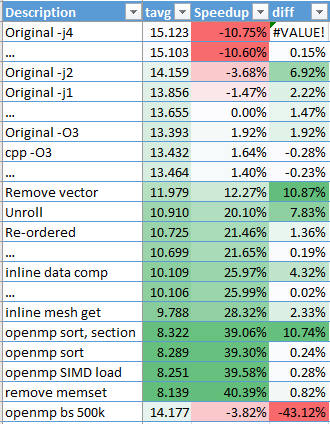
\includegraphics[width=\columnwidth]{data_log}
	\caption{The Result of Optimisation}
	\label{fig:log}
\end{figure}


\subsection{Result validation}

Run multiple times, check output...


\subsection{C++ library}

Changed the library to C++ for...
Changing the library to C++ files in order to test whether \texttt{Thread Building Blocks (TBB)} can be used in the optimisation. In addition, the example program is written by C++, and it is more convenient to use lambda function in \texttt{Mesh::find6Neighbours} and \texttt{Mesh::find18Neighbours}. 

\subsection{Remove unnecessary memory allocations}

Removed \texttt{vector} allocation in...

\subsection{Unroll neighbours checking functions}

Removed complex inefficient implementation...

\subsection{Re-order neighbours checks}

Adjacent checks...

Combine checks manually...

Compiler optimisations...

\subsection{Inline simple functions}

Data comparison functions \texttt{Data::less} and \texttt{Data::greater} are moved into header file instead of writing in source file. In addition, the \texttt{Mesh::getNeighbours} are put inline as well. Because those three functions are small and called frequently. Putting them as inline functions will gain higher efficiency. 

\subsection{Parallelise \texttt{createGraph}}

Using openmp to parallel \texttt{sort()} in \texttt{Mesh::createGraph}...
As the result shown on the gprof, the execution time of the \texttt{std::sort} occupies a large percentage of the whole program running time. Paralleling the \texttt{sort} function is an perfect technique to increasing the performance of \texttt{simple}. Finding a exist paralleled sort library from large company is more effective and efficiency approach than building up own paralleled sort library. \cite{parallelsort} The library has a function named as \texttt{pss::parallel\_stable\_sort()}. The arguments input the function are the same as the \texttt{std::sort()}. 

\subsection{Parallelise \texttt{findNeighbours}}

Memory allocation...

Extract...

Reduce memory usage...

Using openmp \cite{dagum1998openmp}...

Manual task blocks...

Failure, not effective.

\subsection{Parallelise \texttt{ct\_sweep}}

Pointers, linked lists, loop parallelisation not possible...

Using openmp sections...

Not effective, slower on some machines...

The loop body only executed once...

\subsection{SIMD implementation of \texttt{Data::load}}

Using SIMD intrinsics...
The load progress can be implemented by SIMD instructions. The \texttt{Data:load} can be optimised by SIMD intrinsics shown in \cite{advnotes}. Firstly, the input data is \texttt{intData} which contain multiple chars (8 bits), however the size of each element from \texttt{intData} is 16 bits. The first 8 bits are invalid. As the result, \texttt{src1, src2} are declared as temporary container for the data. Also, \texttt{\_\_mm\_and\_si128()} will compute the bitwise AND of 128-bit value in two arguments, so that the invalid bit are set to 0. This progress is a preparation for \texttt{\_\_mm\_packus\_epi16()}. This function will pack the 16 signed 16-bit integers from 2 inputs into 8-bit unsigned integers and saturates. That is the reason why set all the invalid bits to 0. In total, there are 16 chars in side one \texttt{pDst}, which means run one time of the loop will load 16 elements, so the times of the loop should be \texttt{totalSize / 16}.
\begin{lstlisting}[caption={Data Load with SIMD Intrinsics},captionpos=b,label=lst:mem]
data = new DataType[totalSize];
__m128i *pDst = (__m128i *) data;
...
__m128i *pSrc = (__m128i *) intData;
for (uint i = 0; i < totalSize / 16; i++) {
	//data[i] = static_cast<DataType>( intData[i] );
	__m128i src1 = _mm_and_si128(*pSrc++, _mm_set1_epi16(0x00ff));
	__m128i src2 = _mm_and_si128(*pSrc++, _mm_set1_epi16(0x00ff));
	*pDst++ = _mm_packus_epi16(src1, src2);
		}
\end{lstlisting}

\subsection{Remove redundant \texttt{memset}}

Redundant \texttt{memset} with \texttt{calloc}...
The function \texttt{calloc} is used to allocate customised size of memory and initialise all bits inside this part of memory into 0. However, \texttt{memset} has the same purpose as the \texttt{calloc}, so it is no need to set all the bits to "0" again. After removing the \texttt{memset}, the total time is decreased by \%0.82 as \fref{fig:log} shows. 

Furthermore, the function \texttt{calloc()} was changed to \texttt{malloc()}, it will not influence the result but the speed is decreased. Although, \texttt{calloc()} will do the memory allocation and memory initialisation together, it is faster than \texttt{malloc()}. The reason for that is \texttt{calloc()} will do less work because it can skip \texttt{memset()} entirely, also it can even not allocate any memory in some cases. Finally, after multiple times testing, \cite{calloc} is not replaced by \texttt{malloc}
%\texttt{calloc} faster than \texttt{malloc}, why...

\subsection{Parallel \texttt{ct\_sweepAndMerge()}}
The longest time consumption is on function \texttt{sweep()}. This function was called twice by two separate functions named as \texttt{ct\_joinSweep()} and \texttt{ct\_splitSweep()}. The argument of those two functions is \texttt{ctx} and when they call \texttt{ct\_sweep}, all the parameters transferred to \texttt{ct\_sweep} are independent which means \texttt{ct\_joinSweep()} and \texttt{ct\_sliptSweep()} can be paralleled. In order to gain better performance, \texttt{parallel sections} are implemented inside of \texttt{ct\_sweepAndMerge} as \lref{lst:secs} shows. The optimisation saves huge part of time as \fref{fig:log} describes. It decreases more than 15\% time compared with last step. 
\begin{lstlisting}[caption={Data Load with SIMD Intrinsics},captionpos=b,label=lst:secs]
ctArc * ct_sweepAndMerge( ctContext * ctx )
{
	ct_checkContext(ctx);
	
#pragma omp parallel sections    
{    
#pragma omp section
    {ct_joinSweep(ctx);}
#pragma omp section
    {ct_splitSweep(ctx);}
}   
    ct_augment( ctx );
    return ctx->tree=ct_merge( ctx );
}
\end{lstlisting}


\subsection{Checking Results with VTune}
VTune was run in the second platform. The first reason is that VTune is a large program so that it take long time to set up. However the primary platform need to have little overhead in order to get accuracy result, so the VTune is install on secondary platform. Furthermore, it is useful to compare the same program running on different processors. After the optimisation, the execution time of program \texttt{simple} is 4.163s on Intel platform. The difference between the time is due to the different processor architectures. The IPC of program running on Intel platform is much higher than AMD platform. 

The last step is checking the achievement of the optimisation. In order to see a obvious result, the largest dataset \texttt{CThead-2by4.256x512x452.uint16} is chosen as the input of program tested by VTune. Those two figures (\fref{fig:noopt} and \fref{fig:opt})below shows how the program  paralleled. There are three colors shown in results which describe how many CPU cores work simultaneously. Red means the program runs in series. Yellow means there are 2 to 6 threads running. Green gives the best result which represents that there are more than 6 Cores work at the same time. The \fref{fig:noopt} describes that the all the functions of the original program run sequentially. The second graph \fref{fig:opt} proves that after optimisation, most of functions are paralleled and the execution time is decreased significantly. 
\begin{figure}[!h]
	\centering
	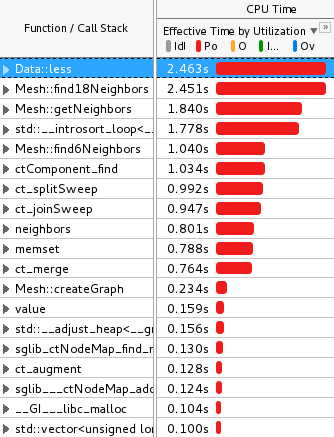
\includegraphics[width=\columnwidth]{noopt_vtune}
	\caption{The Program without Optimisation}
	\label{fig:noopt}
\end{figure}
\begin{figure}[!h]
	\centering
	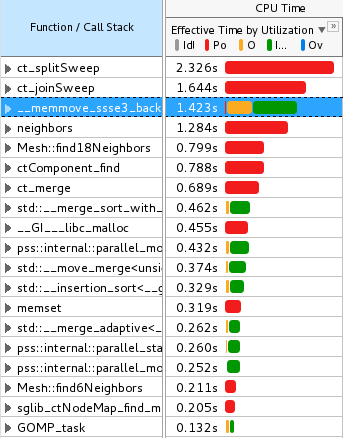
\includegraphics[width=\columnwidth]{opt_vtune}
	\caption{The Final Optimised Program}
	\label{fig:opt}
\end{figure}


\section{Group work}

You may work in groups of two or three if you wish, but your report must include an explicit statement of who did what.

% An example of a floating figure using the graphicx package.
% Note that \label must occur AFTER (or within) \caption.
% For figures, \caption should occur after the \includegraphics.
% Note that IEEEtran v1.7 and later has special internal code that
% is designed to preserve the operation of \label within \caption
% even when the captionsoff option is in effect. However, because
% of issues like this, it may be the safest practice to put all your
% \label just after \caption rather than within \caption{}.
%
% Reminder: the "draftcls" or "draftclsnofoot", not "draft", class
% option should be used if it is desired that the figures are to be
% displayed while in draft mode.
%
%\begin{figure}[!t]
%\centering
%\includegraphics[width=2.5in]{myfigure}
% where an .eps filename suffix will be assumed under latex, 
% and a .pdf suffix will be assumed for pdflatex; or what has been declared
% via \DeclareGraphicsExtensions.
%\caption{Simulation results for the network.}
%\label{fig_sim}
%\end{figure}

% Note that the IEEE typically puts floats only at the top, even when this
% results in a large percentage of a column being occupied by floats.


% An example of a double column floating figure using two subfigures.
% (The subfig.sty package must be loaded for this to work.)
% The subfigure \label commands are set within each subfloat command,
% and the \label for the overall figure must come after \caption.
% \hfil is used as a separator to get equal spacing.
% Watch out that the combined width of all the subfigures on a 
% line do not exceed the text width or a line break will occur.
%
%\begin{figure*}[!t]
%\centering
%\subfloat[Case I]{\includegraphics[width=2.5in]{box}%
%\label{fig_first_case}}
%\hfil
%\subfloat[Case II]{\includegraphics[width=2.5in]{box}%
%\label{fig_second_case}}
%\caption{Simulation results for the network.}
%\label{fig_sim}
%\end{figure*}
%
% Note that often IEEE papers with subfigures do not employ subfigure
% captions (using the optional argument to \subfloat[]), but instead will
% reference/describe all of them (a), (b), etc., within the main caption.
% Be aware that for subfig.sty to generate the (a), (b), etc., subfigure
% labels, the optional argument to \subfloat must be present. If a
% subcaption is not desired, just leave its contents blank,
% e.g., \subfloat[].


% An example of a floating table. Note that, for IEEE style tables, the
% \caption command should come BEFORE the table and, given that table
% captions serve much like titles, are usually capitalized except for words
% such as a, an, and, as, at, but, by, for, in, nor, of, on, or, the, to
% and up, which are usually not capitalized unless they are the first or
% last word of the caption. Table text will default to \footnotesize as
% the IEEE normally uses this smaller font for tables.
% The \label must come after \caption as always.
%
%\begin{table}[!t]
%% increase table row spacing, adjust to taste
%\renewcommand{\arraystretch}{1.3}
% if using array.sty, it might be a good idea to tweak the value of
% \extrarowheight as needed to properly center the text within the cells
%\caption{An Example of a Table}
%\label{table_example}
%\centering
%% Some packages, such as MDW tools, offer better commands for making tables
%% than the plain LaTeX2e tabular which is used here.
%\begin{tabular}{|c||c|}
%\hline
%One & Two\\
%\hline
%Three & Four\\
%\hline
%\end{tabular}
%\end{table}


% Note that the IEEE does not put floats in the very first column
% - or typically anywhere on the first page for that matter. Also,
% in-text middle ("here") positioning is typically not usedpossible, but it
% is allowed and encouraged for Computer Society conferences (but
% not Computer Society journals). Most IEEE journals/conferences use
% top floats exclusively. 
% Note that, LaTeX2e, unlike IEEE journals/conferences, places
% footnotes above bottom floats. This can be corrected via the
% \fnbelowfloat command of the stfloats package.




\section{Conclusion}
The conclusion goes here.

Speed-up achieved... by...

Try other compilers...

GPU acceleration not effective (pointers? linked lists?)


% conference papers do not normally have an appendix


% use section* for acknowledgment
%\section*{Acknowledgment}

%The authors would like to thank...

% trigger a \newpage just before the given reference
% number - used to balance the columns on the last page
% adjust value as needed - may need to be readjusted if
% the document is modified later
%\IEEEtriggeratref{8}
% The "triggered" command can be changed if desired:
%\IEEEtriggercmd{\enlargethispage{-5in}}

% references section

% can use a bibliography generated by BibTeX as a .bbl file
% BibTeX documentation can be easily obtained at:
% http://mirror.ctan.org/biblio/bibtex/contrib/doc/
% The IEEEtran BibTeX style support page is at:
% http://www.michaelshell.org/tex/ieeetran/bibtex/
\bibliographystyle{IEEEtran}
% argument is your BibTeX string definitions and bibliography database(s)
\bibliography{IEEEabrv,references}
%
% <OR> manually copy in the resultant .bbl file
% set second argument of \begin to the number of references
% (used to reserve space for the reference number labels box)
%\begin{thebibliography}{1}

%\bibitem{IEEEhowto:kopka}
%H.~Kopka and P.~W. Daly, \emph{A Guide to \LaTeX}, 3rd~ed.\hskip 1em plus
%  0.5em minus 0.4em\relax Harlow, England: Addison-Wesley, 1999.

%\end{thebibliography}




% that's all folks
\end{document}


